% ------------------------------------------------------------
% LaTeX Template für die DHBW zum Schnellstart!
% Original: https://github.wdf.sap.corp/vtgermany/LaTeX-Template-DHBW
% ------------------------------------------------------------
% ---- Präambel mit Angaben zum Dokument
\documentclass[
	fontsize=12pt,           % Leitlinien sprechen von Schriftgröße 12.
	paper=A4,
	twoside=false,
	listof=totoc,            % Tabellen- und Abbildungsverzeichnis ins Inhaltsverzeichnis
	bibliography=totoc,      % Literaturverzeichnis ins Inhaltsverzeichnis aufnehmen
	titlepage,               % Titlepage-Umgebung anstatt \maketitle
	headsepline,             % horizontale Linie unter Kolumnentitel
	abstract,              % Überschrift einschalten, Abstract muss in {abstract}-Umgebung stehen
]{scrreprt}                  % Verwendung von KOMA-Report
\usepackage[utf8]{inputenc}  % UTF8 Encoding einschalten
\usepackage[ngerman]{babel}  % Neue deutsche Rechtschreibung
\usepackage[T1]{fontenc}     % Ausgabe von westeuropäischen Zeichen (auch Umlaute)
\usepackage{microtype}       % Trennung von Wörtern wird besser umgesetzt
\usepackage{lmodern}         % Nicht-gerasterte Schriftarten (bei MikTeX erforderlich)
\usepackage{graphicx}        % Einbinden von Grafiken erlauben
\usepackage{wrapfig}         % Grafiken fließend im Text
\usepackage{setspace}        % Zeilenabstand \singlespacing, \onehalfspaceing, \doublespacing
\usepackage[
	%showframe,                % Ränder anzeigen lassen
	left=2.7cm, right=2.5cm,
	top=2.5cm,  bottom=2.5cm,
	includeheadfoot
]{geometry}                      % Seitenlayout einstellen
\usepackage{scrlayer-scrpage}    % Gestaltung von Fuß- und Kopfzeilen
\usepackage{acronym}             % Abkürzungen, Abkürzungsverzeichnis
\usepackage{titletoc}            % Anpassungen am Inhaltsverzeichnis
\contentsmargin{0.75cm}          % Abstand im Inhaltsverzeichnis zw. Punkt und Seitenzahl
\usepackage[                     % Klickbare Links (enth. auch "nameref", "url" Package)
  hidelinks,                     % Blende die "URL Boxen" aus.
  breaklinks=true                % Breche zu lange URLs am Zeilenende um
]{hyperref}
\usepackage[hypcap=true]{caption}% Anker Anpassung für Referenzen
\urlstyle{same}                  % Aktuelle Schrift auch für URLs
% Anpassung von autoref für Gleichungen (ergänzt runde Klammern) und Algorithm.
% Anstatt "Listing" kann auch z.B. "Code-Ausschnitt" verwendet werden. Dies sollte
% jedoch synchron gehalten werden mit \lstlistingname (siehe weiter unten).
\addto\extrasngerman{%
	\def\equationautorefname~#1\null{Gleichung~(#1)\null}
	\def\lstnumberautorefname{Zeile}
	\def\lstlistingautorefname{Listing}
	\def\algorithmautorefname{Algorithmus}
	% Damit einheitlich "Abschnitt 1.2[.3]" verwendet wird und nicht "Unterabschnitt 1.2.3"
	% \def\subsectionautorefname{Abschnitt}
}

% ---- Abstand verkleinern von der Überschrift 
\renewcommand*{\chapterheadstartvskip}{\vspace*{.5\baselineskip}}

% Hierdurch werden Schusterjungen und Hurenkinder vermieden, d.h. einzelne Wörter
% auf der nächsten Seite oder in einer einzigen Zeile.
% LaTeX kann diese dennoch erzeugen, falls das Layout ansonsten nicht umsetzbar ist.
% Diese Werte sind aber gute Startwerte.
\widowpenalty10000
\clubpenalty10000

% ---- Für das Quellenverzeichnis
\usepackage[
	backend = biber,                % Verweis auf biber
	language = auto,
	style = numeric,                % Nummerierung der Quellen mit Zahlen
	sorting = none,                 % none = Sortierung nach der Erscheinung im Dokument
	sortcites = true,               % Sortiert die Quellen innerhalb eines cite-Befehls
	block = space,                  % Extra Leerzeichen zwischen Blocks
	hyperref = true,                % Links sind klickbar auch in der Quelle
	%backref = true,                % Referenz, auf den Text an die zitierte Stelle
	bibencoding = auto,
	giveninits = true,              % Vornamen werden abgekürzt
	doi=false,                      % DOI nicht anzeigen
	isbn=false,                     % ISBN nicht anzeigen
    alldates=short                  % Datum immer als DD.MM.YYYY anzeigen
]{biblatex}
\addbibresource{Inhalt/literatur.bib}
\setcounter{biburlnumpenalty}{3000}     % Umbruchgrenze für Zahlen
\setcounter{biburlucpenalty}{6000}      % Umbruchgrenze für Großbuchstaben
\setcounter{biburllcpenalty}{9000}      % Umbruchgrenze für Kleinbuchstaben
\DeclareNameAlias{default}{family-given}  % Nachname vor dem Vornamen
\AtBeginBibliography{\renewcommand{\multinamedelim}{\addslash\space
}\renewcommand{\finalnamedelim}{\multinamedelim}}  % Schrägstrich zwischen den Autorennamen
\DefineBibliographyStrings{german}{
  urlseen = {Einsichtnahme:},                      % Ändern des Titels von "besucht am"
}
\usepackage[babel,german=quotes]{csquotes}         % Deutsche Anführungszeichen + Zitate


% ---- Für Mathevorlage
\usepackage{amsmath}    % Erweiterung vom Mathe-Satz
\usepackage{amssymb}    % Lädt amsfonts und weitere Symbole
\usepackage{MnSymbol}   % Für Symbole, die in amssymb nicht enthalten sind.


% ---- Für Quellcodevorlage
\usepackage{scrhack}                    % Hack zur Verw. von listings in KOMA-Script
\usepackage{listings}                   % Darstellung von Quellcode
\usepackage{xcolor}                     % Einfache Verwendung von Farben
% -- Eigene Farben für den Quellcode
\definecolor{JavaLila}{rgb}{0.4,0.1,0.4}
\definecolor{JavaGruen}{rgb}{0.3,0.5,0.4}
\definecolor{JavaBlau}{rgb}{0.0,0.0,1.0}
\definecolor{ABAPKeywordsBlue}{HTML}{6000ff}
\definecolor{ABAPCommentGrey}{HTML}{808080}
\definecolor{ABAPStringGreen}{HTML}{4da619}
\definecolor{PyKeywordsBlue}{HTML}{0000AC}
\definecolor{PyCommentGrey}{HTML}{808080}
\definecolor{PyStringGreen}{HTML}{008080}
% -- Farben für ABAP CDS
\definecolor{CDSString}{HTML}{FF8C00}
\definecolor{CDSKeywords}{HTML}{6000ff}
\definecolor{CDSAnnotation}{HTML}{00BFFF}
\definecolor{CDSComment}{HTML}{808080}
\definecolor{CDSFunc}{HTML}{FF0000}

% -- Default Listing-Styles

\lstset{
	% Das Paket "listings" kann kein UTF-8. Deswegen werden hier 
	% die häufigsten Zeichen definiert (ä,ö,ü,...)
	literate=%
		{á}{{\'a}}1 {é}{{\'e}}1 {í}{{\'i}}1 {ó}{{\'o}}1 {ú}{{\'u}}1
		{Á}{{\'A}}1 {É}{{\'E}}1 {Í}{{\'I}}1 {Ó}{{\'O}}1 {Ú}{{\'U}}1
		{à}{{\`a}}1 {è}{{\`e}}1 {ì}{{\`i}}1 {ò}{{\`o}}1 {ù}{{\`u}}1
		{À}{{\`A}}1 {È}{{\'E}}1 {Ì}{{\`I}}1 {Ò}{{\`O}}1 {Ù}{{\`U}}1
		{ä}{{\"a}}1 {ë}{{\"e}}1 {ï}{{\"i}}1 {ö}{{\"o}}1 {ü}{{\"u}}1
		{Ä}{{\"A}}1 {Ë}{{\"E}}1 {Ï}{{\"I}}1 {Ö}{{\"O}}1 {Ü}{{\"U}}1
		{â}{{\^a}}1 {ê}{{\^e}}1 {î}{{\^i}}1 {ô}{{\^o}}1 {û}{{\^u}}1
		{Â}{{\^A}}1 {Ê}{{\^E}}1 {Î}{{\^I}}1 {Ô}{{\^O}}1 {Û}{{\^U}}1
		{œ}{{\oe}}1 {Œ}{{\OE}}1 {æ}{{\ae}}1 {Æ}{{\AE}}1 {ß}{{\ss}}1
		{ű}{{\H{u}}}1 {Ű}{{\H{U}}}1 {ő}{{\H{o}}}1 {Ő}{{\H{O}}}1
		{ç}{{\c c}}1 {Ç}{{\c C}}1 {ø}{{\o}}1 {å}{{\r a}}1 {Å}{{\r A}}1
		{€}{{\euro}}1 {£}{{\pounds}}1 {«}{{\guillemotleft}}1
		{»}{{\guillemotright}}1 {ñ}{{\~n}}1 {Ñ}{{\~N}}1 {¿}{{?`}}1,
	breaklines=true,        % Breche lange Zeilen um 
	breakatwhitespace=true, % Wenn möglich, bei Leerzeichen umbrechen
	% Symbol für Zeilenumbruch einfügen
	prebreak=\raisebox{0ex}[0ex][0ex]{\ensuremath{\rhookswarrow}},
	postbreak=\raisebox{0ex}[0ex][0ex]{\ensuremath{\rcurvearrowse\space}},
	tabsize=4,                                 % Setze die Breite eines Tabs
	basicstyle=\ttfamily\small,                % Grundsätzlicher Schriftstyle
	columns=fixed,                             % Besseres Schriftbild
	numbers=left,                              % Nummerierung der Zeilen
	%frame=single,                             % Umrandung des Codes
	showstringspaces=false,                    % Keine Leerzeichen hervorheben
	keywordstyle=\color{blue},
	ndkeywordstyle=\bfseries\color{darkgray},
	identifierstyle=\color{black},
	commentstyle=\itshape\color{JavaGruen},   % Kommentare in eigener Farbe
	stringstyle=\color{JavaBlau},             % Strings in eigener Farbe,
	captionpos=b,                             % Bild*unter*schrift
	xleftmargin=5.0ex
}

% ---- Eigener JAVA-Style für den Quellcode
\renewcommand{\ttdefault}{pcr}               % Schriftart, welche auch fett beinhaltet
\lstdefinestyle{EigenerJavaStyle}{
	language=Java,                             % Syntax Highlighting für Java
	%frame=single,                             % Umrandung des Codes
	keywordstyle=\bfseries\color{JavaLila},    % Keywords in eigener Farbe und fett
	commentstyle=\itshape\color{JavaGruen},    % Kommentare in eigener Farbe und italic
	stringstyle=\color{JavaBlau}               % Strings in eigener Farbe
}

% ---- Eigener ABAP-Style für den Quellcode
\renewcommand{\ttdefault}{pcr}
\lstdefinestyle{EigenerABAPStyle}{
	language=[R/3 6.10]ABAP,
	morestring=[b]\|,                          % Für Pipe-Strings
	morestring=[b]\`,                          % für Backtick-Strings
	keywordstyle=\bfseries\color{ABAPKeywordsBlue},
	commentstyle=\itshape\color{ABAPCommentGrey},
	stringstyle=\color{ABAPStringGreen},
	tabsize=2,
	morekeywords={
		types,
		@data,
		as,
		lower,
		start,
		selection,
		order,
		by,
		inner,
		join,
		key,
		end,
		cast
	}
}

% ---- Eigener Python-Style für den Quellcode
\renewcommand{\ttdefault}{pcr}
\lstdefinestyle{EigenerPythonStyle}{
	language=Python,
	columns=flexible,
	keywordstyle=\bfseries\color{PyKeywordsBlue},
	commentstyle=\itshape\color{PyCommentGrey},
	stringstyle=\color{PyStringGreen}
}

%----- ABAP-CDS-View language
\lstdefinelanguage{ABAPCDS}{
	sensitive=false,
	%Keywords
	morekeywords={define,
		view,
		as,
		select,
		from,
		inner,
		join,
		on,
		key,
		case,
		when,
		then,
		else,
		end,
		true,
		false,
		cast,
		where,
		and,
		distinct,
		group,
		by,
		having,
		min,
		sum,
		max,
		count,
		avg
	},
	%Methoden
	morekeywords=[2]{
		div,
		currency\_conversion,
		dats\_days\_between,
		concat\_with\_space,
		dats\_add_days,
		dats\_is\_valid,
		dats\_add\_months,
		unit\_conversion,
		division,
		mod,
		abs,
		floor,
		ceil,
		round,
		concat,
		replace,
		substring,
		left,
		right,
		length
	},
	morecomment=[s][\color{CDSAnnotation}]{@}{:},
	morecomment=[l][\itshape\color{CDSComment}]{//},
	morecomment=[s][\itshape\color{CDSComment}]{/*}{*/},
	morestring=[b][\color{CDSString}]',
	keywordstyle=\bfseries\color{CDSKeywords},
	keywordstyle=[2]\color{CDSFunc}
}

  % Weitere Details sind ausgelagert

\usepackage{algorithm}                  % Für Algorithmen-Umgebung (ähnlich wie lstlistings Umgebung)
\usepackage{algpseudocode}              % Für Pseudocode. Füge "[noend]" hinzu, wenn du kein "endif",
                                        % etc. haben willst.

\makeatletter                           % Sorgt dafür, dass man @ in Namen verwenden kann.
                                        % Ansonsten gibt es in der nächsten Zeile einen Compilefehler.
\renewcommand{\ALG@name}{Algorithmus}   % Umbenennen von "Algorithm" im Header der Listings.
\makeatother                            % Zeichen wieder zurücksetzen
\renewcommand{\lstlistingname}{Listing} % Erlaubt das Umbenennen von "Listing" in anderen Titel.

% ---- Tabellen
\usepackage{booktabs}  % Für schönere Tabellen. Enthält neue Befehle wie \midrule
\usepackage{multirow}  % Mehrzeilige Tabellen
\usepackage{siunitx}   % Für SI Einheiten und das Ausrichten Nachkommastellen
\sisetup{locale=DE, range-phrase={~bis~}, output-decimal-marker={,}} % Damit ein Komma und kein Punkt verwendet wird.
\usepackage{xfrac} % Für siunitx Option "fraction-function=\sfrac"

% ---- Für Definitionsboxen in der Einleitung
\usepackage{amsthm}                     % Liefert die Grundlagen für Theoreme
\usepackage[framemethod=tikz]{mdframed} % Boxen für die Umrandung
% ---- Definition für Highlight Boxen

% ---- Grundsätzliche Definition zum Style
\newtheoremstyle{defi}
  {\topsep}         % Abstand oben
  {\topsep}         % Abstand unten
  {\normalfont}     % Schrift des Bodys
  {0pt}             % Einschub der ersten Zeile
  {\bfseries}       % Darstellung von der Schrift in der Überschrift
  {:}               % Trennzeichen zwischen Überschrift und Body
  {.5em}            % Abstand nach dem Trennzeichen zum Body Text
  {\thmname{#3}}    % Name in eckigen Klammern
\theoremstyle{defi}

% ------ Definition zum Strich vor eines Texts
\newmdtheoremenv[
  hidealllines = true,       % Rahmen komplett ausblenden
  leftline = true,           % Linie links einschalten
  innertopmargin = 0pt,      % Abstand oben
  innerbottommargin = 4pt,   % Abstand unten
  innerrightmargin = 0pt,    % Abstand rechts
  linewidth = 3pt,           % Linienbreite
  linecolor = gray!40,       % Linienfarbe
]{defStrich}{Definition}     % Name der des formats "defStrich"

% ------ Definition zum Eck-Kasten um einen Text
\newmdtheoremenv[
  hidealllines = true,
  innertopmargin = 6pt,
  linecolor = gray!40,
  singleextra={              % Eck-Markierungen für die Definition
    \draw[line width=3pt,gray!50,line cap=rect] (O|-P) -- +(1cm,0pt);
    \draw[line width=3pt,gray!50,line cap=rect] (O|-P) -- +(0pt,-1cm);
    \draw[line width=3pt,gray!50,line cap=rect] (O-|P) -- +(-1cm,0pt);
    \draw[line width=3pt,gray!50,line cap=rect] (O-|P) -- +(0pt,1cm);
  }
]{defEckKasten}{Definition}  % Name der des formats "defEckKasten"  % Weitere Details sind ausgelagert

% ---- Für Todo Notes
\usepackage{todonotes}
\setlength {\marginparwidth }{2cm}      % Abstand für Todo Notizen


% ---- Elektronische Version oder Gedruckte Version?
% ---- Unterschied: Die elektronische Version enthält keinen Platzhalter für die Unterschrift
\usepackage{ifthen}
\newboolean{e-Abgabe}
\setboolean{e-Abgabe}{false}    % false=gedruckte Fassung

% ---- Persönlichen Daten:
\newcommand{\titel}{Morik Password Manager}
\newcommand{\titelheader}{Morik}
\newcommand{\arbeit}{Programmentwurf}
\newcommand{\studiengang}{Informatik}
\newcommand{\studienjahr}{2019}
\newcommand{\autorOne}{Moritz Gutfleisch}
\newcommand{\autorTwo}{Erik Zimmermann}
\newcommand{\autorReverse}{Nachname, Vorname}
\newcommand{\verfassungsort}{Karlsruhe}
\newcommand{\matrikelnrOne}{9540703}
\newcommand{\matrikelnrTwo}{2152543}
\newcommand{\kurs}{TINF19B1}
\newcommand{\bearbeitungsmonat}{Januar 2018}
\newcommand{\abgabe}{30. April 2022}
\newcommand{\bearbeitungszeitraum}{04.10.2021 - 30.04.2022}
\newcommand{\betreuerDhbw}{Daniel Lindner}

% ---- Metainformation für das PDF Dokument
\hypersetup{
	pdftitle    = {\titel},
	pdfsubject  = {\arbeit},
	pdfauthor   = {\autorOne{}, \autorTwo{}},
	%pdfkeywords = {Keywords angeben},
	pdfcreator  = {LaTeX},
	%pdfproducer = {in der Regel pdfTeX}
}

% ---- Definition der Kopf- und Fußzeilen
\clearscrheadfoot                               % Löschen von LaTeX Standard
\automark[section]{chapter}                     % Füllen von section und chapter
\renewcommand*{\chaptermarkformat}{}            % Entfernt die Kapitelnummer
\renewcommand*{\sectionmarkformat}{}            % Entfernt die Sectionnummer
% Angaben [für "plain"]{für "scrheadings"}
\ihead[]{\titelheader}                          % Kopfzeile links
\chead[]{}                                      % Kopfzeile mitte
\ohead[]{\rightmark}                            % Kopfzeile rechts
\ifoot[]{}                                      % Fußzeile links
\cfoot*{\sffamily\pagemark}                     % Fußzeile mitte
\ofoot[]{}                                      % Fußzeile rechts
\KOMAoptions{
   headsepline = 0.2pt,                         % Liniendicke Kopfzeile
   footsepline = false                          % Liniendicke Fußzeile
}

% ---- Hilfreiches
\newcommand{\zB}{z.\,B. }   % "z.B." mit kleinem Leeraum dazwischen (ohne wäre nicht korrekt)
\newcommand{\dash}{d.\,h. }

\newcommand{\code}[1]{\texttt{#1}} % Ist einfacher zu schreiben als ständig \texttt und erlaubt
                                   % Änderungen im Nachhinein, wenn man z.B. Inline-Code anders stylen möchte.

% ---- Silbentrennung (falls LaTeX defaults falsch / nicht gewünscht sind)
\hyphenation{HANA}         % anstatt HA-NA
\hyphenation{Graph-Script} % anstatt GraphS-cript

% ---- Beginn des Dokuments
\begin{document}
\setlength{\parindent}{0pt}              % Keine Paragraphen Einrückung.
                                         % Dafür haben wir den Abstand zwischen den Paragraphen.
\setcounter{secnumdepth}{2}              % Nummerierungstiefe fürs Inhaltsverzeichnis
\setcounter{tocdepth}{1}                 % Tiefe des Inhaltsverzeichnisses. Ggf. so anpassen,
                                         % dass das Verzeichnis auf eine Seite passt.
\sffamily                                % Serifenlose Schrift verwenden.

% ---- Vorspann
% ------ Titelseite
\singlespacing
\thispagestyle{empty}
\begin{titlepage}
\enlargethispage{4cm}

\vspace*{0.1cm}

\begin{center}
	\Huge{\textbf{\titel}}\\[1.5cm]
	\LARGE{\textbf{\arbeit}}\\[1cm]
	\normalsize{von}\\[1ex] \Large{\textbf{\autorOne}} \\[1ex]
	\normalsize{und}\\[1ex] \Large{\textbf{\autorTwo}} \\[1cm]
\end{center}

\begin{center}
	\vfill
	\begin{tabular}{ll}
		Abgabedatum:                     & \abgabe \\[0.2cm]
		Bearbeitungszeitraum:            & \bearbeitungszeitraum \\[0.2cm]
		Matrikelnummer, Student:            & \matrikelnrOne{}, \autorOne \\[0.2cm]
		Matrikelnummer, Student:            & \matrikelnrTwo{}, \autorTwo \\[0.2cm]
		Kurs:            & \kurs \\[0.2cm]
		Gutachter der Dualen Hochschule: & \betreuerDhbw \\[2cm]
	\end{tabular} 
\end{center}
\end{titlepage}
  % Titelseite
\newcounter{savepage}
\pagenumbering{Roman}                    % Römische Seitenzahlen
\onehalfspacing

% ------ Inhaltsverzeichnis
\singlespacing
\tableofcontents

% ------ Verzeichnisse
\renewcommand*{\chapterpagestyle}{plain}
\pagestyle{plain}
\listoffigures                          % Erzeugen des Abbildungsverzeichnisses 
\listoftables                           % Erzeugen des Tabellenverzeichnisses
\setcounter{savepage}{\value{page}}


% ---- Inhalt der Arbeit
\cleardoublepage
\pagenumbering{arabic}                  % Arabische Seitenzahlen für den Hauptteil
\setlength{\parskip}{0.5\baselineskip}  % Abstand zwischen Absätzen
\rmfamily
\renewcommand*{\chapterpagestyle}{scrheadings}
\pagestyle{scrheadings}
\onehalfspacing
\chapter{Einleitung}
\chapter{Clean Architecture}
\section{Plugins}
\subsection{Datenbank}
Die Datenbank stellt eines der Plugins dar. Als Technologie wurde hier eine SQLite3 Datenbank verwendet. Die konkrete Implementierung der Schnittstelle zur SQLite-Datenbank befindet sich in der Klasse \href{https://github.com/moorts/Morik/blob/main/src/plugins/database/SQLiteDatabase.h}{\textit{SQLiteDatabase}}. Diese Klasse erbt von der abstrakten Klasse \href{https://github.com/moorts/Morik/blob/main/src/application/AbstractDatabase.h}{\textit{AbstractDatabase}}, die sich in der Applikationsschicht befindet. Hierdurch wird eine Dependency Inversion erreicht, da nun eine \textit{AbstractDatabase} von anderen Klassen verwendet werden kann, um SQL-Befehle auf der Datenbank auszuführen, statt eine konkrete \textit{SQLiteDatabase} zu verwenden, was die Abhängigkeit von innen nach außen laufen lassen würde.

\subsection{Verschlüsselung}

Ein weiteres Plugin ist die Verschlüsselungsbibliothek. Als solche wurde Cryptopp\footnote{\url{https://cryptopp.com/}} verwendet. Die abstrakte Klasse \href{https://github.com/moorts/Morik/blob/main/src/application/Cipher.h}{\textit{Cipher}} definiert die Schnittstelle in der Applikationsschicht, die das Plugin implementieren muss. Eine konkrete Implementierung dieser Schnittstelle befindet sich in der Klasse \href{https://github.com/moorts/Morik/blob/main/src/plugins/encryption/CBC\_Cipher.h}{\textit{CBC\_Cipher}}. Dadurch findet auch hier eine Dependency Inversion statt, da \textit{Cipher} verwendet werden kann, um Verschlüsselung zu verwenden, statt eine Dependency auf eine konkrete Klasse der Pluginschicht zu brauchen. Die Schnittstelle muss lediglich einen String ver- und entschlüsseln können unter Angabe des Klar- bzw. Geheimtextes und eines Schlüssels. \textit{CBC\_Cipher} implementiert dies für die Chiffren, die im \href{https://github.com/moorts/Morik/blob/main/src/plugins/encryption/BLOCK.h}{\textit{BLOCK}} enum aufgezählt sind. Momentan handelt es sich dabei um AES und Serpent, neue Chiffren können allerdings leicht hinzugefügt werden, solange sie von Cryptopp unterstützt werden. Diese werden als Block-Chiffren mit Cipher Block Chaining (CBC) als Betriebsmodus verwendet. Um andere Betriebsmodi, oder Nicht-Blockchiffren zu verwenden, müssten weitere Implementierungen des \textit{Cipher} Interfaces hinzugefügt werden. Dies ist ohne Weiteres möglich, solange ein \textit{String} zür Schlüsselherleitung hinreichend ist.

\section{Adapter}
\subsection{Datenbank}
Die Klasse \href{https://github.com/moorts/Morik/blob/main/src/application/DbInterface.h}{\textit{DbInterface}} implementiert die eigentliche Funktionalität in Form der SQL-Anweisungen und führt diese über eine konkrete Implementierung der \textit{AbstractDatabase} in der Datenbank aus. Somit geht keine Funktionalität verloren, wenn das Plugin durch eine andere Datenbanktechnologie ausgetauscht wird. Die Umsetzung der Funktionalität als SQL-Anweisungen bedeutet jedoch, dass ein Austausch des Plugins nur ohne Weiteres möglich ist, wenn die neue Datenbank ebenfalls eine SQL-Datenbank ist. Handelt es sich bei der neuen Datenbank jedoch beispielsweise um eine noSQL-Datenbank, so muss die Funktionalität, also die Abfragen, angepasst werden. Der Klasse \textit{DbInterface} wird im Konstruktor eine \textit{AbstractDatabase} übergeben, was die Dependency Injection umsetzt.\\
Auf die Benutzung von Prepared Statements wurde innerhalb des Adapters verzichtet, da die Datenbank lokal ist und nur der Benutzer Befehle auf ihr ausführt. Würde die Datenbank über eine öffentliche Schnittstelle angesteuert werden, so wäre dies nicht zu vernachlässigen.

\chapter{Programming Principles}
\chapter{Domain Driven Design}
\section{Ubiquitous Language}

\begin{table}[t]
	\centering
	\noindent\makebox[\textwidth]{
		\begin{tabular}{ c | c }
			Domänenexperte (KeePass/1Password) & Implementierung (Morik) \\
			\hline
			Password & PlaintextPassword \\
			Password & EncryptedPassword \\
			Entry/Item & Entry \\
			UUID & EntryId \\ 
			Title & EntryName \\
			User Name & Login \\
			Vault & EntryRepository \\
			Password Generator & PasswordGenerator \\
			? & PasswordEncrypter \\
			? & PasswordDecryper \\
		\end{tabular}
	}
	\caption{Ubiquitous Language Gegenüberstellung}
	\label{tab:ubiquitous_language}
\end{table}

Die Analyse der Ubiquitous Language ergab die zuvor genannten Programmteile, deren Bezeichnungen mit denen anderer Passwortmanager verglichen werden. KeePass unterscheidet in der Ubiquitous Language nicht zwischen den zwei von uns identifizierten Arten von Passwörtern, nämlich PlaintextPassword und EncryptedPassword. Stattdessen werden diese zwei Umstände meist mit Adverben beschrieben ("sensitive data is stored encryptedly", "make sensitive data available unencryptedly") oder mithilfe mehrerer Substantive ("passwords as plain-text"). Da wir im Source Code weder mit Adverben noch mit unnötig langen Konstrukten aus mehreren Substantiven arbeiten wollen, wir jedoch trotzdem eine Unterscheidung der beiden Zustände eines Passworts benötigen, haben wir uns für die beiden genannten Varianten entschieden. Was das Entry angeht, so verwenden wir den gleichen Begriff wie KeePass (1Password zieht hier Item vor). Was die EntryId angeht, so verwenden wir keine UUID, da wir nur Entries verwalten und demnach keine eindeutige Kennung über mehrere Tabellen hinweg benötigen. Das Präfix "Entry" vor der Id dient dem besseren Nachvollziehen von was es die Id ist. Das Gleiche gilt für das Präfix des EntryName. Hier haben wir uns für Name statt wie KeePass für Title entschieden, da wir dies für eindeutiger halten. Außerdem haben wir uns gegen User Name entschieden und haben stattdessen Login gewählt als Begriff, da unser Passwort Manager darauf abzielt dem Benutzer beim Anmelden zu helfen. Aus diesem Grund kann im Feld Login die konkrete Zeichenkette gespeichert werden, die der Benutzer zum Anmelden braucht, sei es tatsächlich der Benutzername oder aber die Email Adresse. Entsprechend uneingeschränkt sollte auch die Bezeichnung dieses Feldes sein, was bei User Name nicht der Fall ist. 1Password nennt den Ort, an dem die Passwörter gespeichert werden den Vault. Wir haben uns stattdessen für EntryRepository entschieden, um zum einen klar zu machen, dass es sich um einen Aufbewahrungsort handelt und zum anderen eindeutig festzulegen, dass dies der Aufbewahrungsort speziell für Entries ist. Dies beseitigt sämtliche Fragen, was genau dort aufbewahrt wird. Beim PasswordGenerator jedoch sind wir uns einig mit der Bezeichnung von KeePass. Weder KeePass noch 1Password benennen die Teile ihrer Software, die die Daten ver- und entschlüsseln. Stattdessen ist die Rede von "encrypted data" und "decrypted data". Da Passwörter die einzigen Felder sind, die von uns ver- und entschlüsselt werden, haben wir uns dafür entschieden die dafür zuständigen Programmteile mit PasswordEncryptor und PasswordDecryptor zu bezeichnen, sodass wir trotzdem die von KeePass und 1Password verwendeten Wortstämme verwenden, daraus jedoch Substantive machen.  

Um die Ubiquitous Language des Programms auch außerhalb des Source Codes zu verwenden, haben wir ebenfalls die Spalten der Datenbank an die festgelegten Begriffe angepasst. Dies kann in \autoref{fig:DDDDatabase} beobachtet werden.

\begin{figure}[ht]
	\centering
	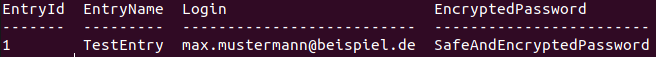
\includegraphics[width=1.0\textwidth]{Bilder/DDD_column_names.png}
	\caption{Datenbank-Spaltennamen nach Ubiquitous Language}
	\label{fig:DDDDatabase}
\end{figure}

\section{Value Objects}
Das erste Value Object ist das PlaintextPassword, welches das vom Benutzer eingegebene abzulegende Passwort beinhaltet bevor es verschlüsselt wird beziehungsweise nachdem es entschlüsselt wird. Es handelt sich dabei um ein Value Object, da es sich um das gleiche PlaintextPassword handelt wenn der Benutzer zwei mal die gleiche Zeichenkette eingibt. Das EncryptedPassword, das das Passwort beinhaltet nachdem es verschlüsselt ist, gilt ebenfalls als Value Object. Dies gilt aus dem gleichen Grund wie beim PlaintextPassword, also dass die gleiche Zeichenkette auch die Gleichheit des Objekts impliziert. Außerdem gilt der EntryName als Value Object, der den Namen, welchen der Benutzer für den Eintrag vergibt, speichert. Hierbei handelt es sich ebenfalls um ein Value Object, da die gleiche eingegebene Zeichenkette bedeutet, dass es sich um den gleichen Namen für den Eintrag handelt. Auch der vom Benutzer optional hinzugefügte Login eines Entrys gilt als Value Object, ebenfalls aus dem Grund dass die gleiche Zeichenkette bedeutet, dass das Objekt das Gleiche ist. Zu guter Letzt gilt auch die EntryId als Value Object, die die ID des Entrys speichert. Hier gilt, dass der gleiche Integer Wert schlussfolgern lässt, dass es das gleiche Objekt der Klasse EntryId ist.

\section{Entities}
Ein Entry beschreibt einen konreten Eintrag in der Datenbank. Der Entry beinhaltet die ID des Eintrags, den Namen des Eintrags, einen optionalen Login und das verschlüsselte Passwort. Man stelle sich Folgendes vor. Der Benutzer löscht einen Entry und erstellt danach einen neuen. Bei dem neuen Entry vergibt er den gleichen Namen, Login und das gleiche Passwort wie bei dem zuvor gelöschten Entry. Handelt es sich darum um den selben Entry? Nein, denn der wurde gelöscht. Darum ist der Entry eine Entity und kein Value Object.

\section{Aggregate}
Es gibt genau ein Aggregat. Dieses Aggregat beinhaltet ein Entry, eine EntryId, einen EntryName, einen Login und ein EncryptedPassword. Diese Teile sind als Aggregat zu betrachten, da sie immer gemeinsam von Interesse sind. Ein Benutzer möchte nicht einfach irgend ein Passwort wissen ohne den zugehörigen Namen des Eintrags zu kennen. Die Aggregat-Root ist dabei der Entry, wobei über die EntryId des Entrys auf das jeweilige Aggregat zugegriffen wird.

\section{Repositories}
Da es nur ein Aggregat gibt, gibt es ebenfalls genau eine Repository. Diese Repository ist die EntryRepository und stellt den Zugriff auf die Datenbank dar, die die Einträge des Benutzers persistiert. Die EntryRepository liefert demnach vorhandene Entries zurück, speichert neue Entries, löscht nicht mehr benötigte und passt Werte eines Entrys an neue Werte an.

\section{Domain Services}
Der Generator für neue Passwörter (PasswordGenerator), sowie die Verschlüsselung eines PlaintextPasswords (PasswordEncryptor) und die Entschlüsselung eines EncryptedPasswords (PasswordDecryptor) werden als Domain Services realisiert.

\chapter{Unit Tests}
\chapter{Entwurfsmuster}
\section{Factory Method}
Das Entwurfsmuster der Factory Method wird von der EntryFactory umgesetzt. Um ein Entry aus den Standarddatentypen zu erzeugen hat die EntryFactory zwei verschiedene statische Factorymethoden. Die Methode \textit{createEntry} nimmt alle notwendigen Daten als Standarddatentyp, also die EntryId als unsigned int, den EntryName, Login und EncryptedPassword als string, und erzeugt daraus die notwendigen Value Objects, um letztendlich den Entry zu erzeugen. Die Methode \textit{createEntryFromPlaintext} hingegen nimmt ebenfalls alle vier notwendigen Parameter als Standarddatentypen entgegen, geht jedoch davon aus, dass das Passwort nicht verschlüsselt ist, weshalb vorerst ein PlaintextPassword aus dem übergebenen String erzeugt wird, das dann an den PasswordEncryptor Domain Service übergeben wird, um ein EncryptedPassword zu erzeugen. Schließlich wird auch hier ein Entry aus den erzeugten Value Objects erzeugt und zurückgegeben. Die EntryFactory vereinfacht also das Erzeugen von Entries dadurch, dass nicht immer erst alle vier Value Objects, die notwendig sind um den Konstruktor des Entrys aufzurufen, erzeugt werden müssen, sondern direkt als Standarddatentyp übergeben werden können und die Factory diese Umwandlung intern vornimmt. Eine Visualisierung der EntryFactory in Form eines UML-Diagramms kann in \autoref{fig:EntryFactory} betrachtet werden.\\

\begin{figure}[ht]
	\centering
	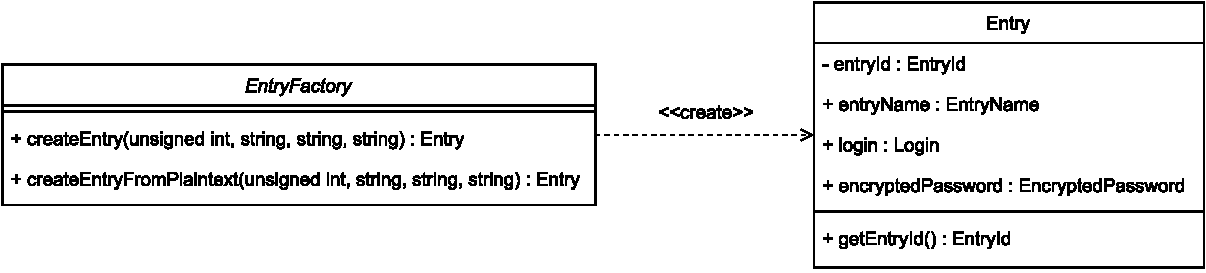
\includegraphics[width=1.0\textwidth]{Bilder/EntryFactory.pdf}
	\caption{UML-Diagramm EntryFactory}
	\label{fig:EntryFactory}
\end{figure}

\chapter{Refactoring}
\label{chap:refactoring}
In diesem Kapitel werden einige der gefundenen Code Smells und der angewendeten Refactorings in Morik erklärt. Bei den Code Smells handelt es sich dabei um verbesserungswürdige Codestellen, während die Refactorings konkrete Lösungen für solche Stellen bieten, ohne dabei das externe Verhalten, wie beispielsweise die Schnittstelle oder die Bedeutung des Ergebnisses, zu verändern.

\section{Code Smells}
\subsection{Duplicated Code}
Bei dem ersten identifizierten Code Smell handelt es sich um duplicated code, also doppelt vorhandenen Code. Dies führt dazu, dass Änderungen an einer Stelle nichts an der Funktionsweise der anderen Stellen ändert, was mehrfachen Pflegeaufwand zur Folge hat. Der Code Smell kann in \href{https://github.com/moorts/Morik/blob/8c90c65347f25b5a5a26f68c66189984dfb0bca6/src/adapters/database/DatabaseInterface.cpp}{dieser Version des DatabaseInterfaces} gesehen werden. Es geht dabei um den Codeabschnitt, der prüft, ob beim Ausführen des SQL-Statements ein Fehler aufgetreten ist. Dieser Codeabschnitt ist in den Methoden \textit{insertEntry} (Z. 30-34), \textit{removeEntry} (Z. 41-45) und \textit{modifyEntry} (Z. 53-57) vorhanden.

\subsection{Long Method}
Ein weiterer Code Smell, der in Morik vorhanden ist, ist long method, also eine lange Klassenmethode. Dieser Code Smell ist in der Methode \textit{mainloop} der Klasse \href{https://github.com/moorts/Morik/blob/main/src/plugins/ui/CommandLineInterface.cpp}{\textit{CommandLineInterface}} zu beobachten, die über 200 Zeilen lang ist.

\subsection{Switch Statement}
Der dritte Code Smell, der gefunden wurde, ist das Switch Statement. Dieses ist nicht flexibel, da es ausschließlich in-place wachsen kann und hat außerdem eine fehleranfällige Syntax, da sehr leicht das \textit{break} am Ende eines Falls vergessen werden kann, was dazu führt, dass mehrer Fälle ausgeführt werden. Dieser Code Smell wurde ebenfalls in der \textit{mainloop}-Methode der \textit{CommandLineInterface}-Klasse gefunden und ist in \href{https://github.com/moorts/Morik/blob/5fad45957d77585d88bf3330cab6004315e6e2e3/src/plugins/ui/CommandLineInterface.cpp#L27}{Zeile 27} zu sehen.

\section{Refactorings}
\subsection{Extract Method}
Das erste Refactoring beseitigt den ersten Code Smell, also den duplicated code im DatabaseInterface. Um dies zu beheben wurde das Refactoring Extract Method angewendet, was in \href{https://github.com/moorts/Morik/commit/09ea85004227950dbf7d30e7bb6de26f92b1ea85}{diesem Commit} beobachtet werden kann, wodurch der duplizierte Code in eine private Methode namens \textit{executeWithErrorCheck} ausgelagert wurde. Das Refactoring führt dazu, dass zukünftig nur noch eine zentrale Stelle anzupassen ist, sollte das Verhalten bei einem Fehler verändert werden müssen. Entsprechend ist nur noch eine Änderung notwendig und jede Codestelle, die die Funktion aufruft ändert sich gleichermaßen. Der Pflegeaufwand nimmt also stark ab, während das Ausführen des Codes einheitlicher abläuft.

\subsection{Rename Method}
Ein weiteres Refactoring, das angewendet wurde ist Rename Method. Dies wurde in \href{https://github.com/moorts/Morik/commit/e807014b1ae894640a8a87f2765fa2ba5d95ea19}{diesem Commit} durchgeführt und sorgt für eindeutigere Namen der Methoden. Der Leser dieser drei Methodenaufrufe muss demnach nicht mehr die Parameter inspizieren, um herauszufinden welche der drei Methoden tatsächlich aufgerufen wird, sondern kann dies direkt am Methodennamen erkennen und weiß daher schneller welches Feld des Entrys bei der betrachteten Codestelle modifiziert wird.


% ---- Literaturverzeichnis
\cleardoublepage
\renewcommand*{\chapterpagestyle}{plain}
\pagestyle{plain}
\pagenumbering{Roman}                   % Römische Seitenzahlen
\setcounter{page}{\numexpr\value{savepage}+1}
\printbibliography[title=Literaturverzeichnis]

% ---- Anhang
\appendix
%\clearpage
%\pagenumbering{Roman}  % römische Seitenzahlen für Anhang

\newpage
\end{document}
